\subsection{Application aux réseaux de régulation}



\subsection{Exemple de méthodes : TIGRESS et GENIE3}
	
	\begin{frame}{TIGRESS : approche basée sur la régression linéaire}

TIGRESS fait le choix de modélisation suivant : l'expression d'un gène cible peut être modélisée par une c\textbf{ombinaison linéaire} de l'expression des facteurs de transcription :
    \onslide<2->
    
    \begin{equation*}
    	   target_i = \textcolor{orange}{\beta_{target,1}}.TF1_i + \textcolor{orange}{\beta_{target,2}}.TF2_i + ... + \textcolor{orange}{\beta_{target,M}}.TFM_i  + \epsilon_i
    \end{equation*}
    
Avec $TFM_i$ le niveau d'expression du TF numéro M dans la condition $i$.
\vspace{0.3cm}

\onslide<3-> 

\begin{alertblock}{\small Problème : il faut \textbf{refléter la sparsité du problème biologique}}
\small L'expression d'un gène est sensée être expliquée par un nombre limité de TFs, et non tous les TFs du jeu de données $\rightarrow$ \textbf{LARS} (Least-angle regression)
\end{alertblock}

\end{frame}



\begin{frame}{TIGRESS : Modéliser la sparsité}

\begin{alertblock}{\small Problème : il faut \textbf{refléter la sparsité du problème biologique}}
\small L'expression d'un gène est sensée être expliquée par un nombre limité de TFs, et non tous les TFs du jeu de données $\rightarrow$ \textbf{LARS} (Least-angle regression)
\end{alertblock}

\scriptsize
La méthode LARS fonctionne (dans le principe) comme suit :

\begin{enumerate}\small 
    \item Commencer par le modèle nul : $target_i = \alpha + \epsilon_i$
    \item Choisir le $TF_j$ pour lequel la corrélation à $target$ est maximale : $target_i = \alpha + \textcolor{orange}{\beta_{target,j}}.TFj_i + \epsilon_i$
    \item Continuer à ajouter des TFs en choisissant à chaque fois le TF maximisant la prédiction de $target$
    \item S'arrêter lorsque l'on a atteint le nombre de TFs prédicteurs jugé suffisant, ici $L < M$.
\end{enumerate}

\scriptsize
On termine alors avec le modèle suivant, consitué de uniquement L TFs contre M, sans contrainte de spasite : 
 $target_i = \textcolor{orange}{\beta_{target,1}}.TF1_i + \textcolor{orange}{\beta_{target,2}}.TF2_i + ... + \textcolor{orange}{\beta_{target,L}}.TFL_i  + \epsilon_i$


\end{frame}
	
\begin{frame}{TIGRESS : étapes de la procédure}
	\vspace{-0.3cm}
	\begin{overprint}
	 \onslide<1> 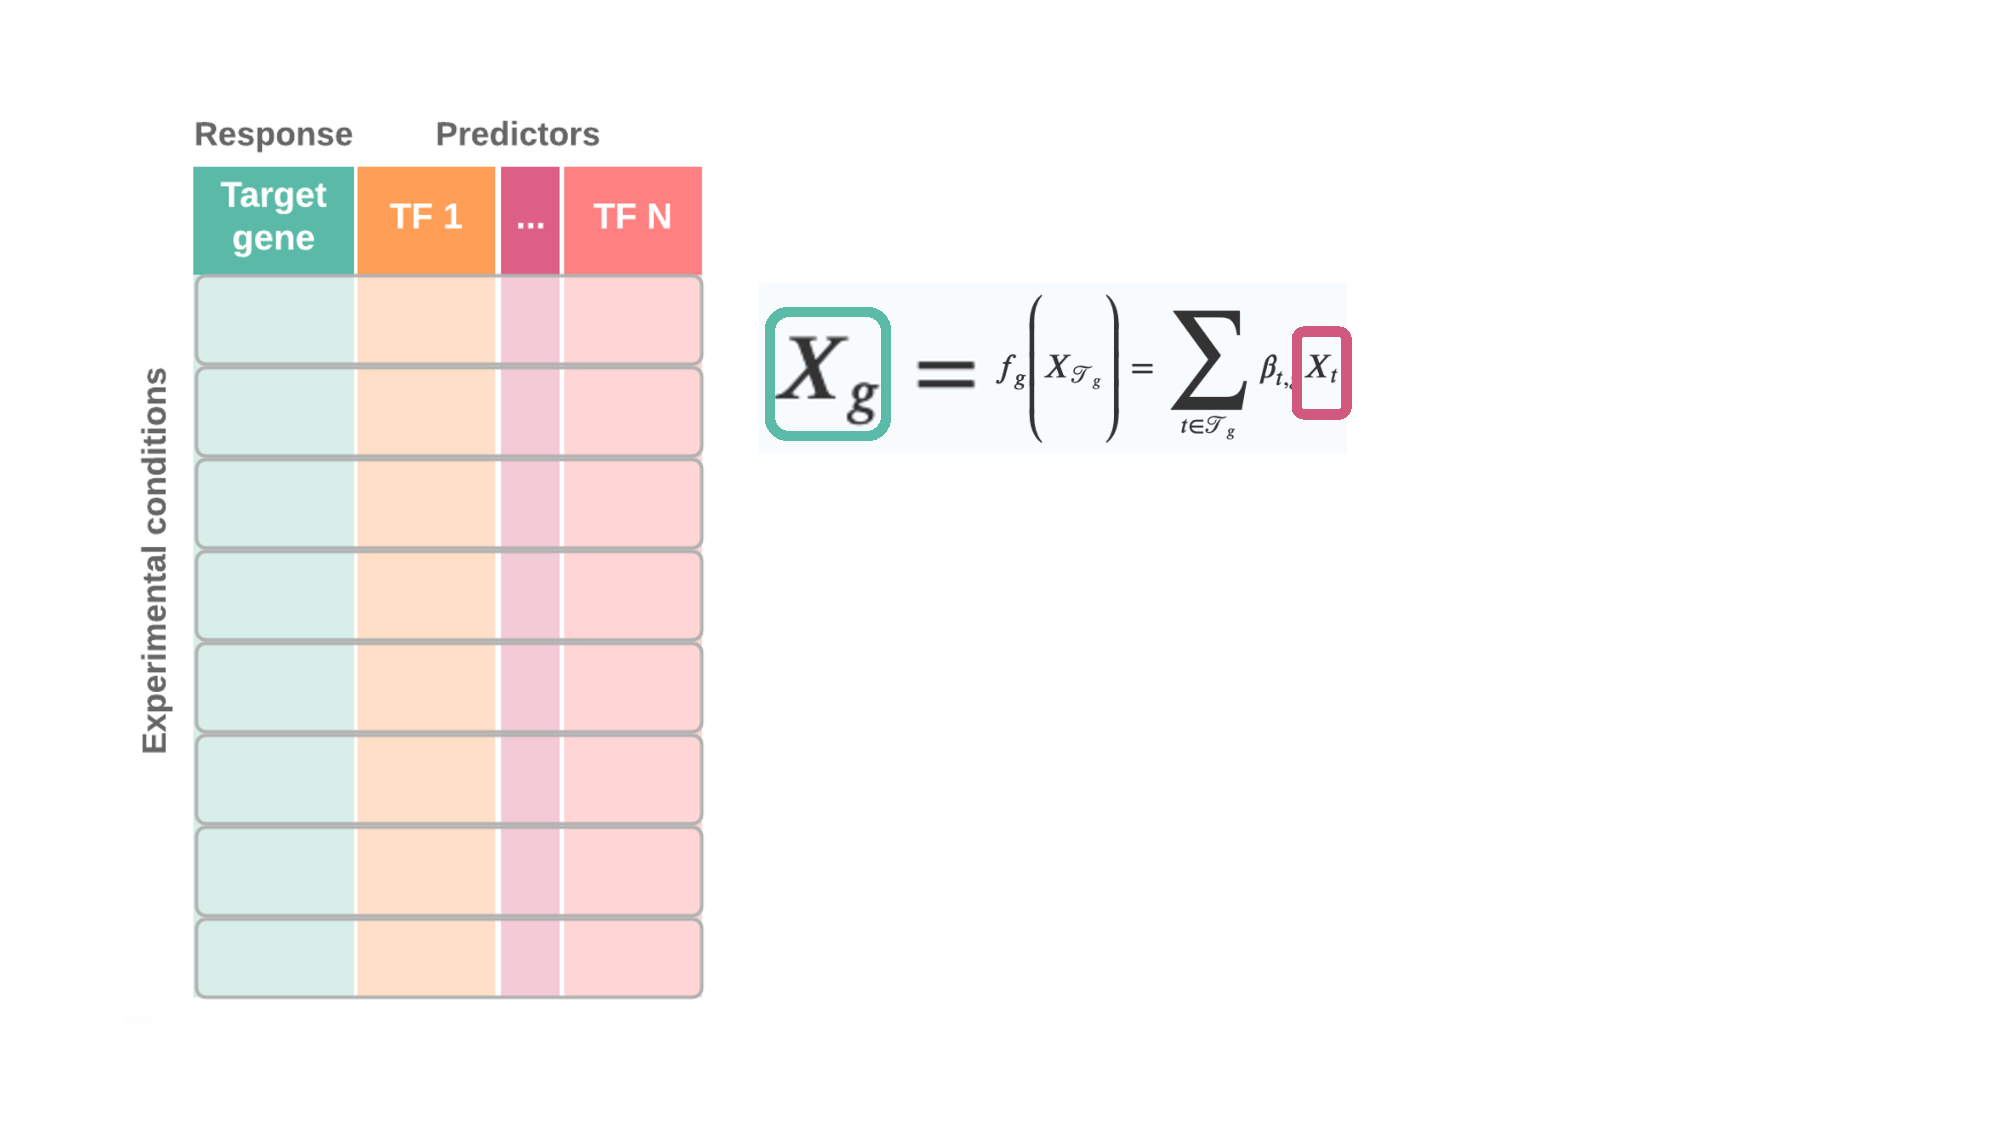
\includegraphics[scale=0.35]{Figures/Regression/tigress_1-1.pdf}
	 \onslide<2> 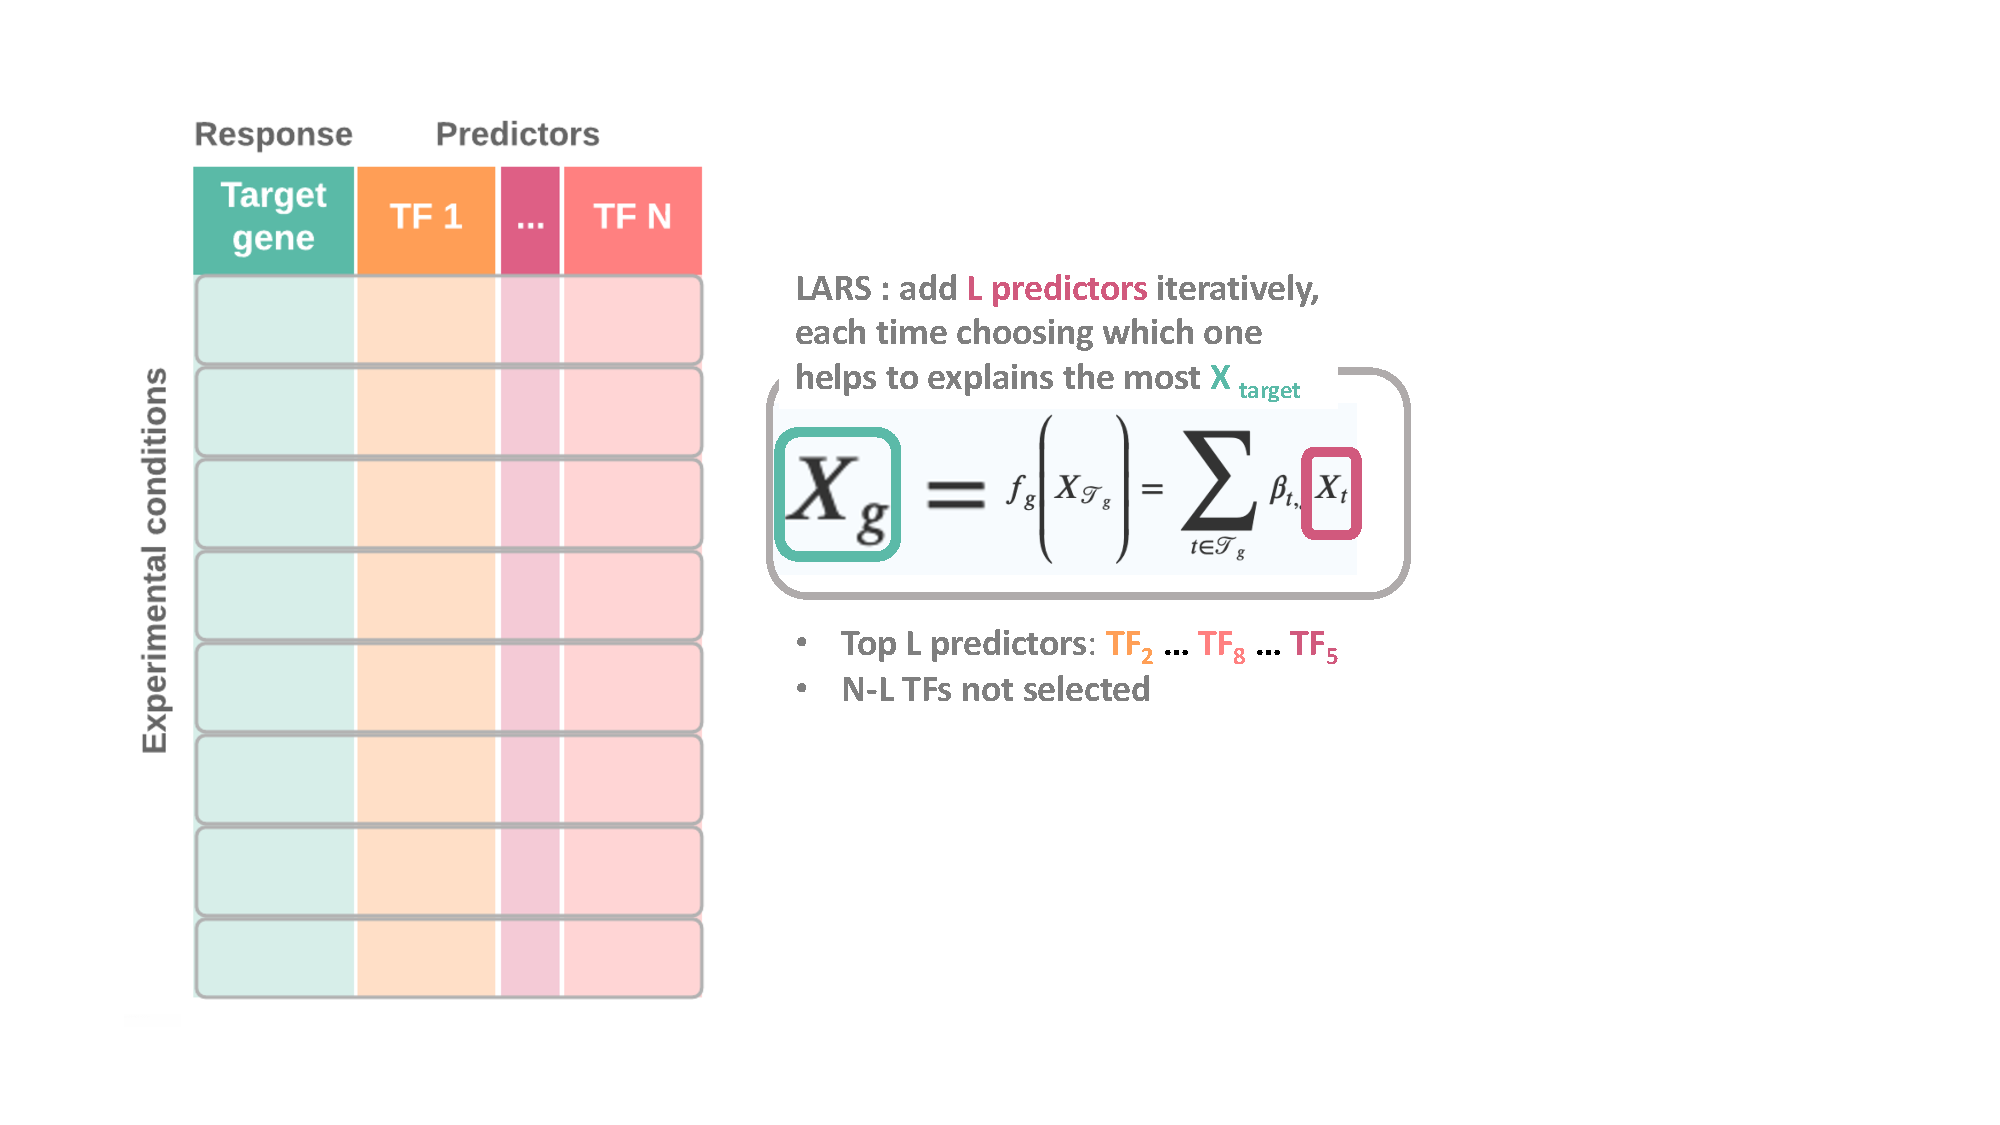
\includegraphics[scale=0.35]{Figures/Regression/tigress_2-2.pdf}
	 \onslide<3> 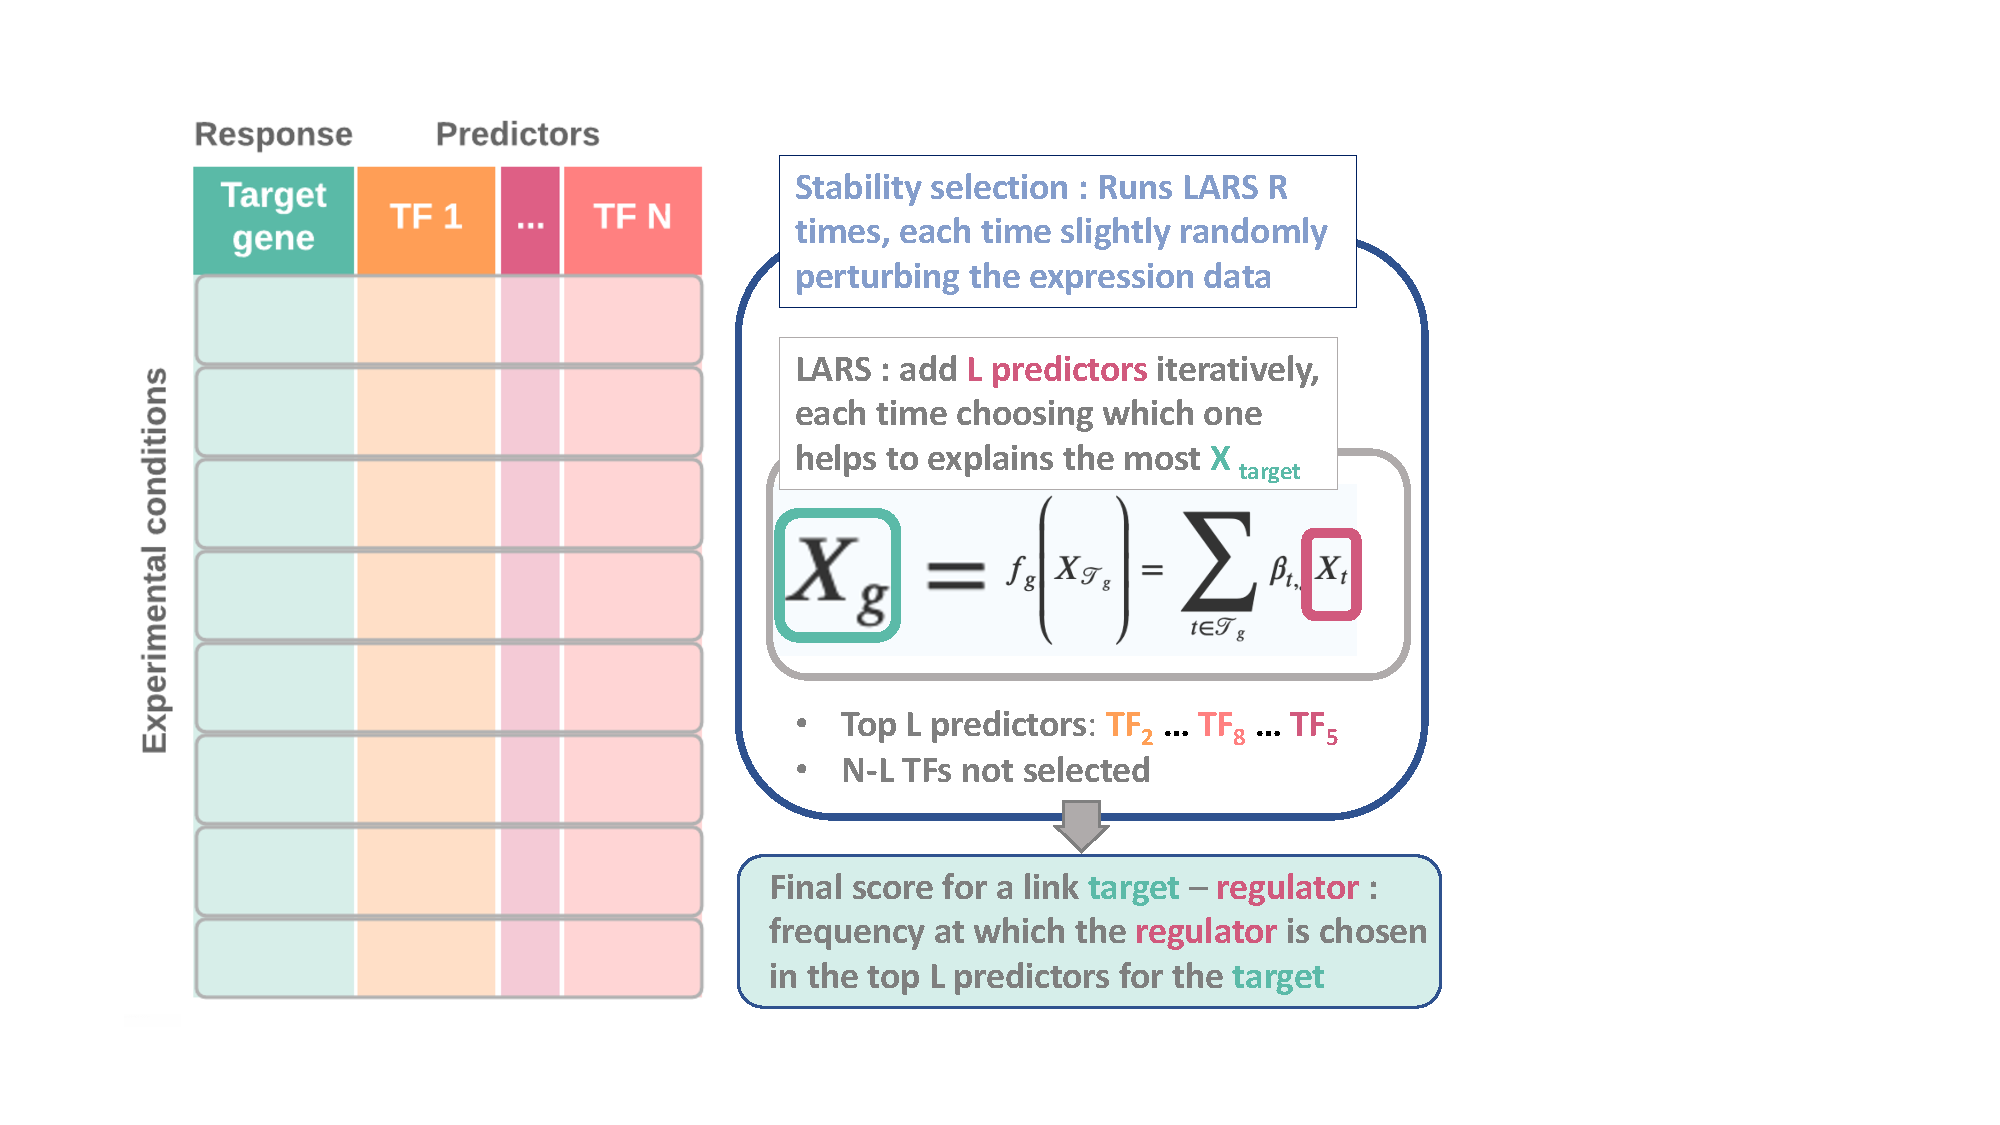
\includegraphics[scale=0.35]{Figures/Regression/tigress_3-3.pdf}
	 \onslide<4> 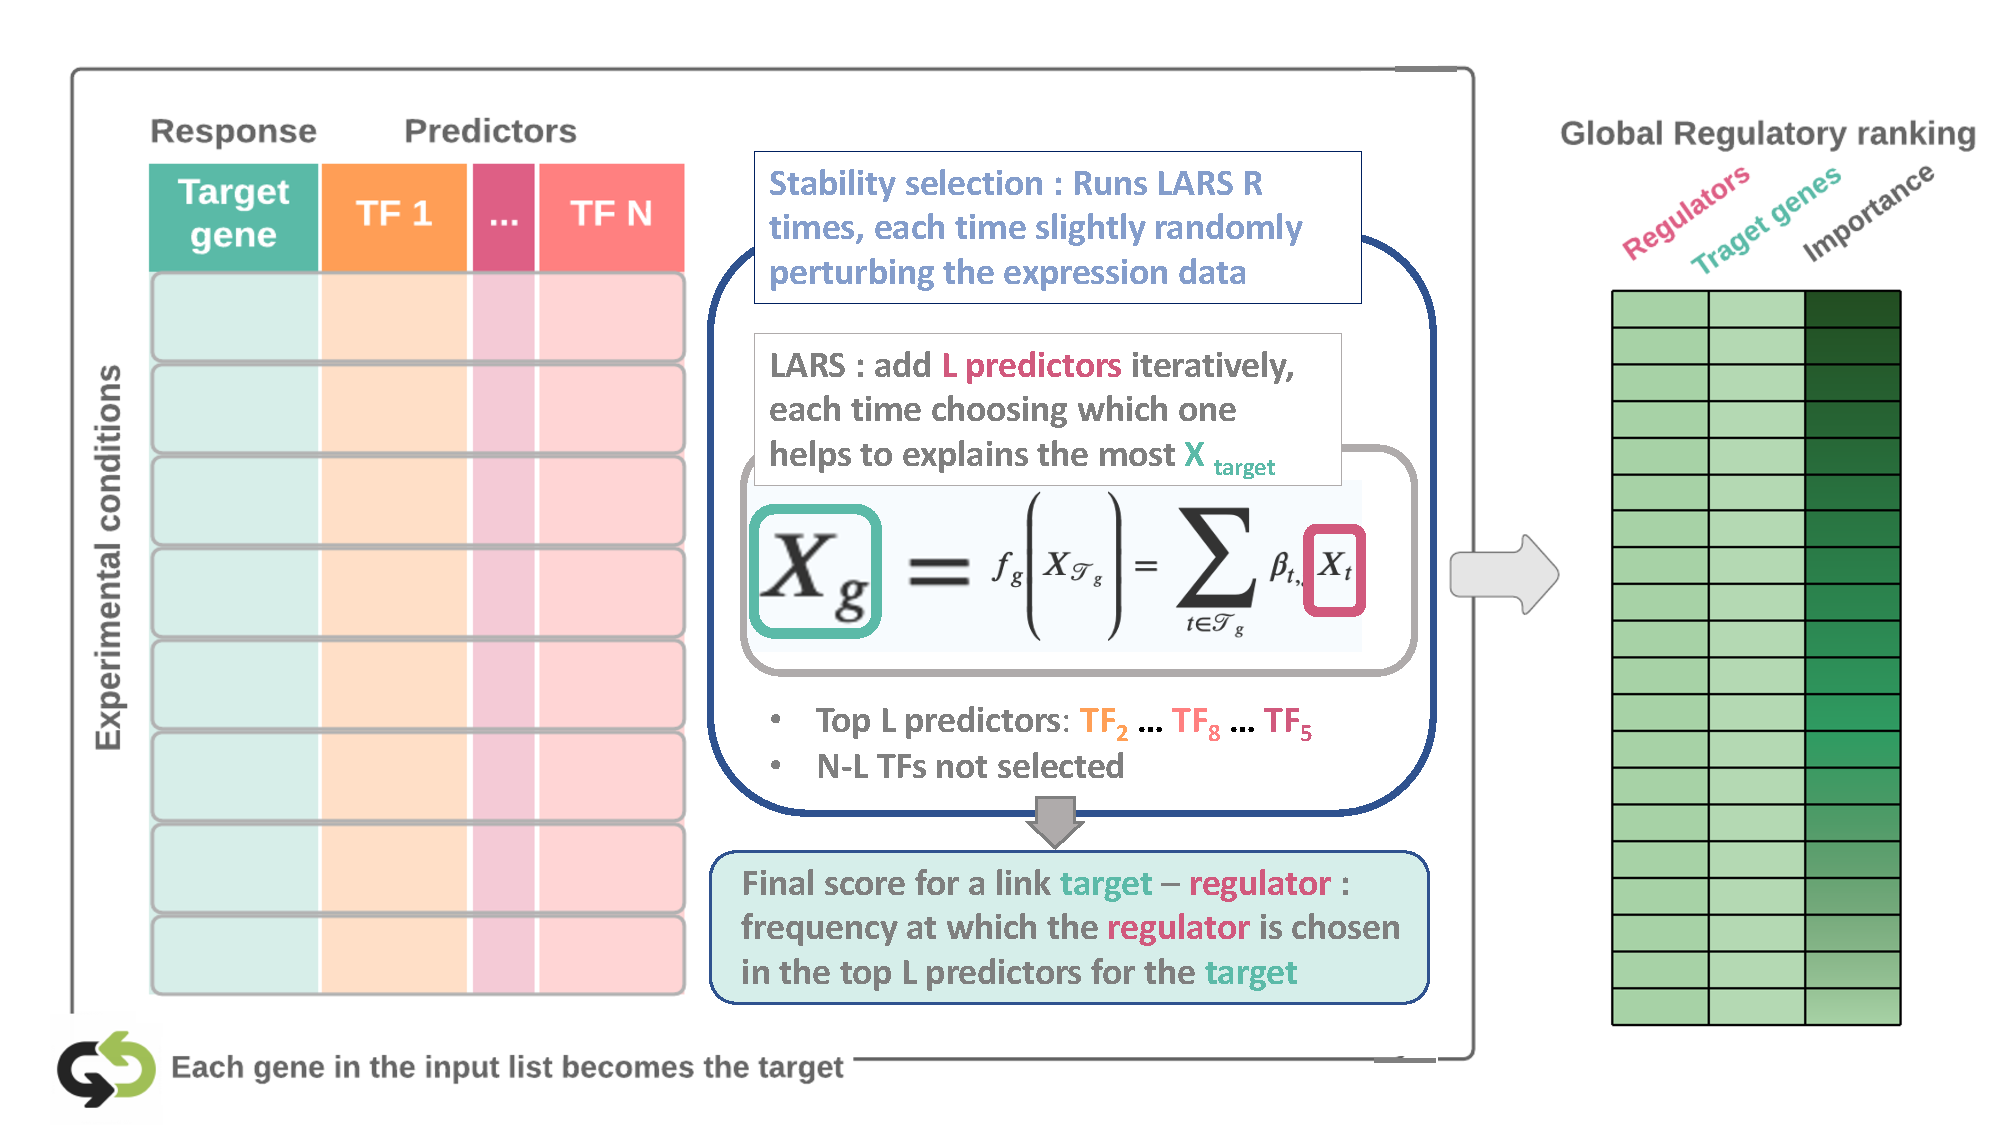
\includegraphics[scale=0.35]{Figures/Regression/tigress_4-end.pdf}
	 
	\end{overprint}
\end{frame}
	
	










\begin{frame}{GENIE3 : approche basée sur les arbres de régression}

GENIE3 fait le choix de modélisation suivant : l'expression d'un gène cible peut être modélisée par une \textbf{combinaison non linéaire} de l'expression des facteurs de transcription :

    \onslide<2->
    
    \begin{equation*}
    	   target_i = \textcolor{orange}{Random Forest}(TF_i) + \epsilon_i
    \end{equation*}
\scriptsize{(On n'a pas de formulation mathématique pour le modèle d'un random forest, qui fonctionne très différemment d'une régression linéaire)}

\small 
Avec $TF_i$ le niveau d'expression de tous les TFs du jeu de données dans la condition $i$.



\begin{block}{\small Avantages par rapport au modèle linéaire}
\begin{itemize}\scriptsize
    \item Peut modéliser des non linéarités dans l'influence de l'expression des régulateurs (ex: le carré de l'expression d'un régulateur, etc)
    \item Peut modéliser des relations de coopération et d'interactions entre TFs
\end{itemize}
\end{block}

\end{frame}



\begin{frame}{GENIE3 : approche basée sur les arbres de régression}


\small Un arbre de régression est construit en choisissant \textbf{des seuils et conditions sur les variables prédictives}.
%Le choix des conditions et seuils sur les variables est fait itérativment, en maximisant la réduction de variabilité de la variable réponse engendrée par l'ajout d'une coniditon.

\begin{columns}
\begin{column}{.45\textwidth}
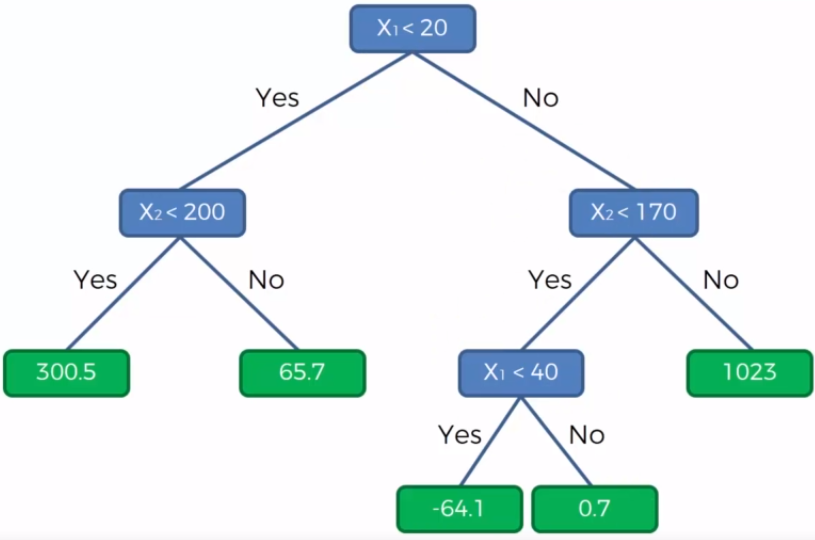
\includegraphics[scale = 0.2]{Figures/Regression/regressionTree.png}
\end{column}
\begin{column}{.45\textwidth}
\small Ajustement d'un arbre de régression
\begin{enumerate}\scriptsize
    \item Choisir la variable et la condition sur cette variable qui permettent de discriminer au mieux les valeurs de la réponse (la variance de la réponse est diminuée)
    \item Réitérer en créant de nouvelles branches, jusqu'à épuisement des variables, ou atteinte de la profondeur d'arbre maximale
\end{enumerate}
\end{column}
\end{columns}
\vspace{0.5cm}

\onslide<2>
\scriptsize \textbf{Random Forest} : un grand nombre d'arbres de régression sont ajustés sur des données échantillonnées légèrement différemment les unes des autres $\rightarrow$ leur consensus permet plus de robustesse dans les prédictions (apprentissage ensembliste)

\end{frame}



\begin{frame}
    \frametitle{GENIE3: étapes de la procédure}
    \small \textbf{Ranking the regulators} according to their \textbf{relevance for predicting} the other genes expression
    \vspace{-0.2cm}
    \begin{center}
        \begin{overprint}
        \onslide<1>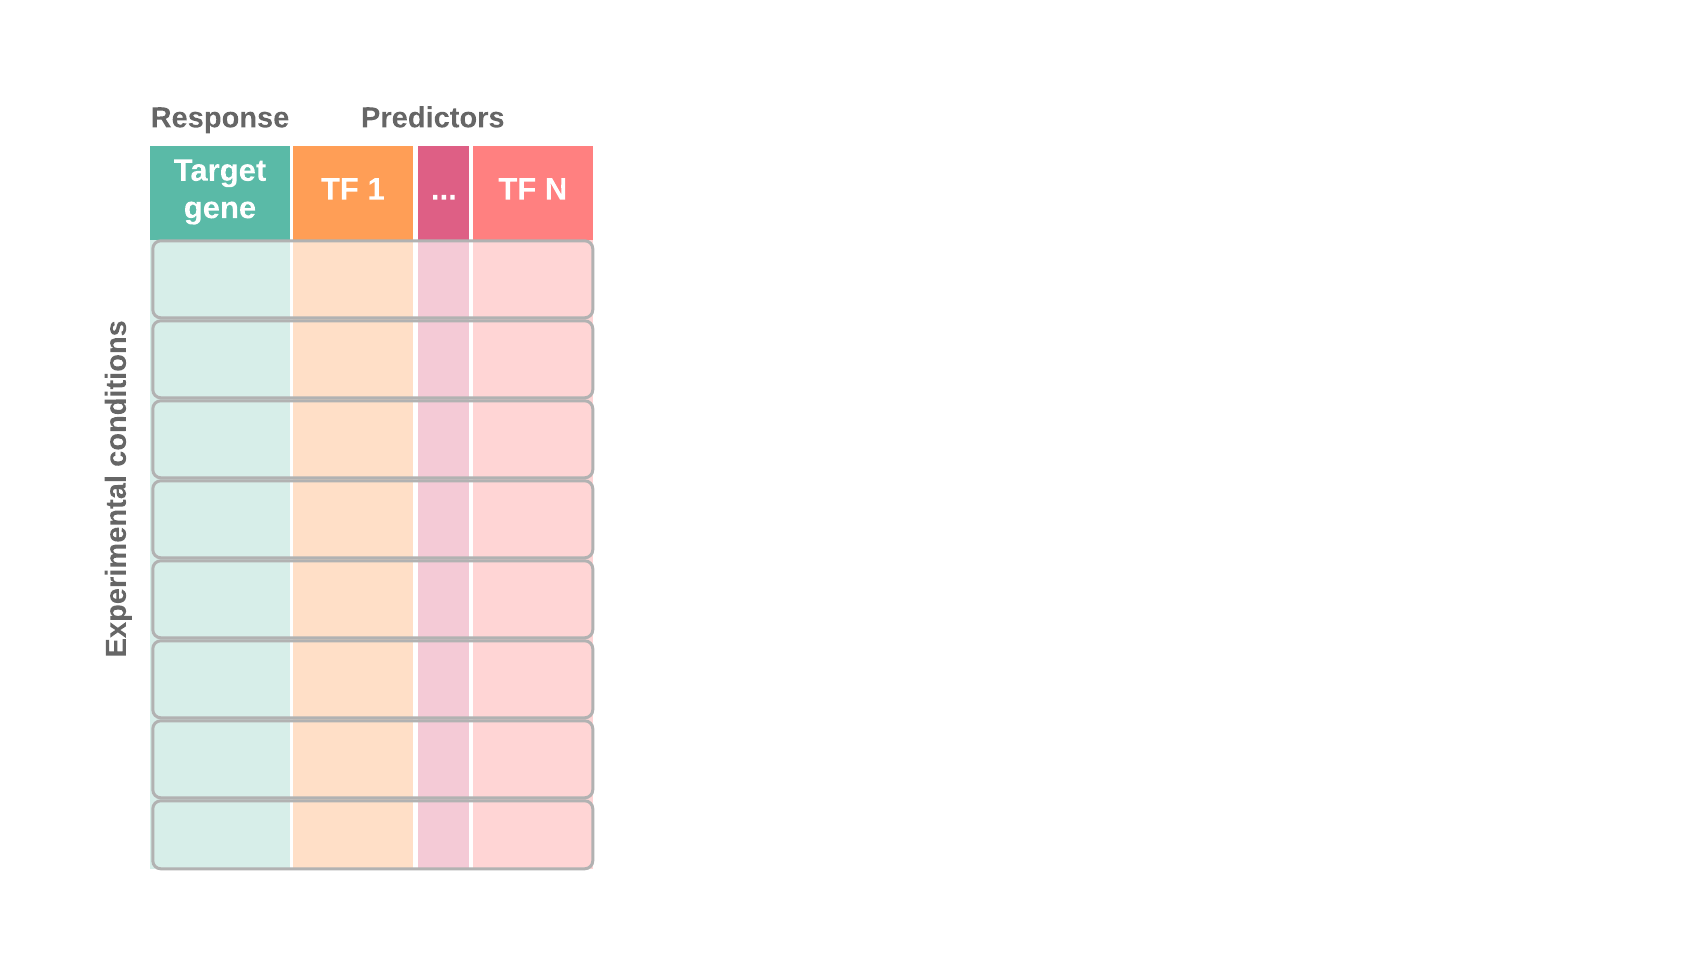
\includegraphics[scale = 0.38]{Figures/Regression/rf1.png}
        \onslide<2>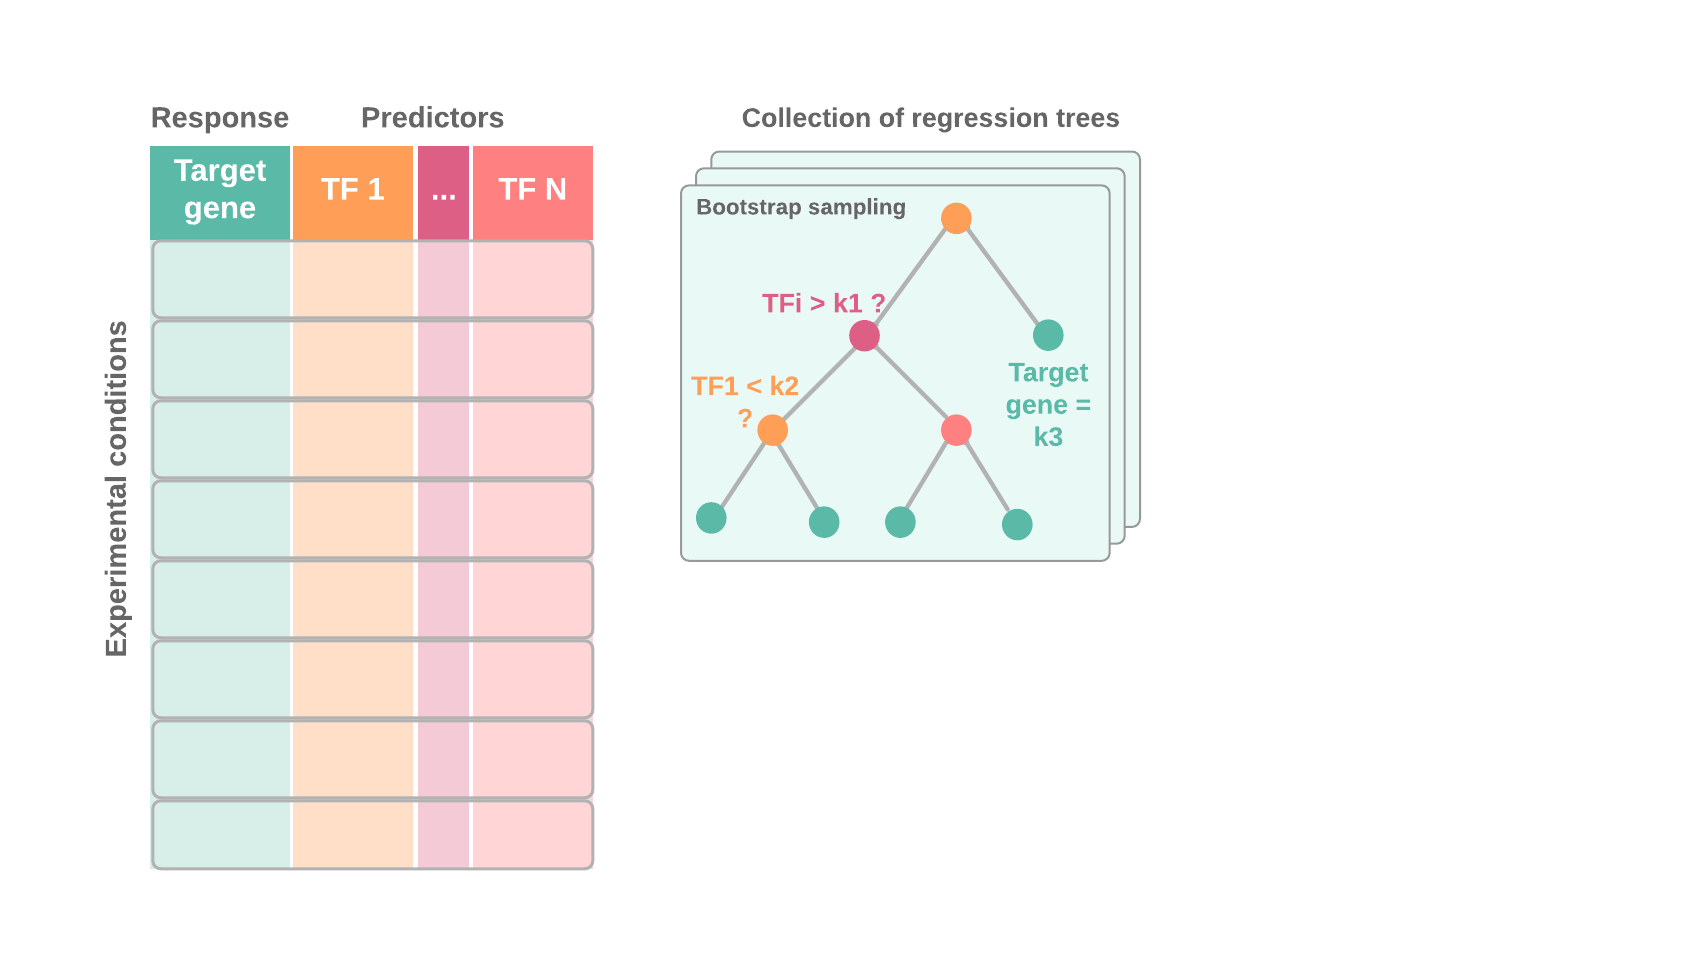
\includegraphics[scale = 0.38]{Figures/Regression/rf2.png}
        \onslide<3>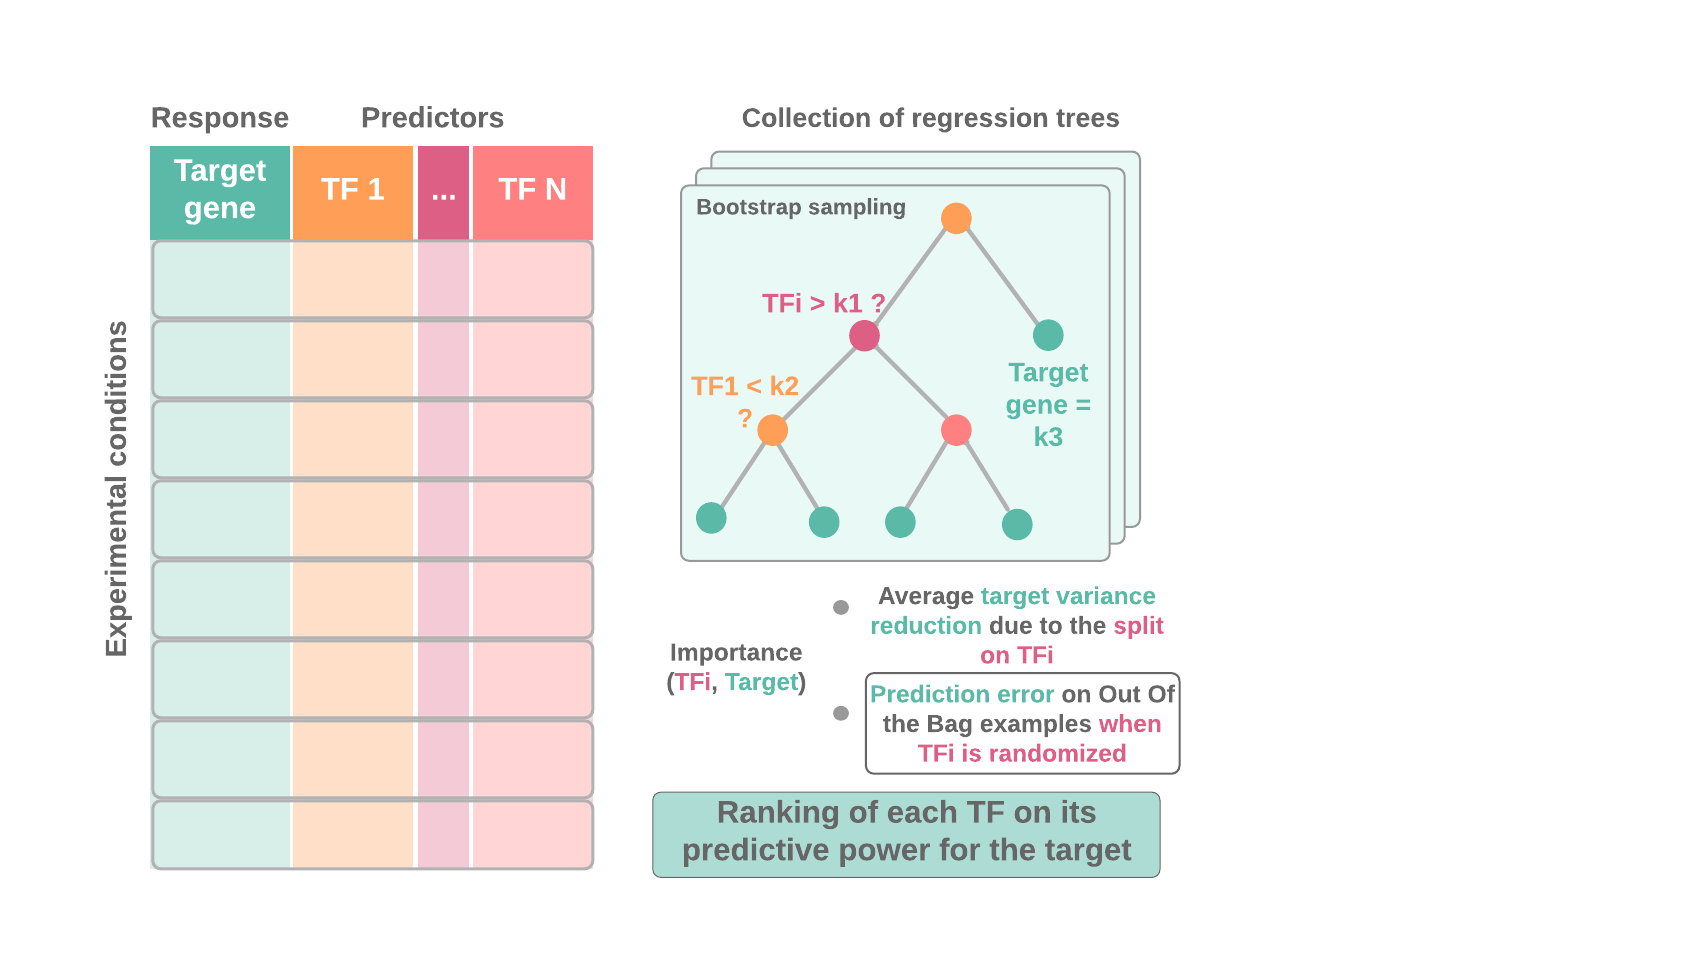
\includegraphics[scale = 0.38]{Figures/Regression/rf3.png}
        \onslide<4->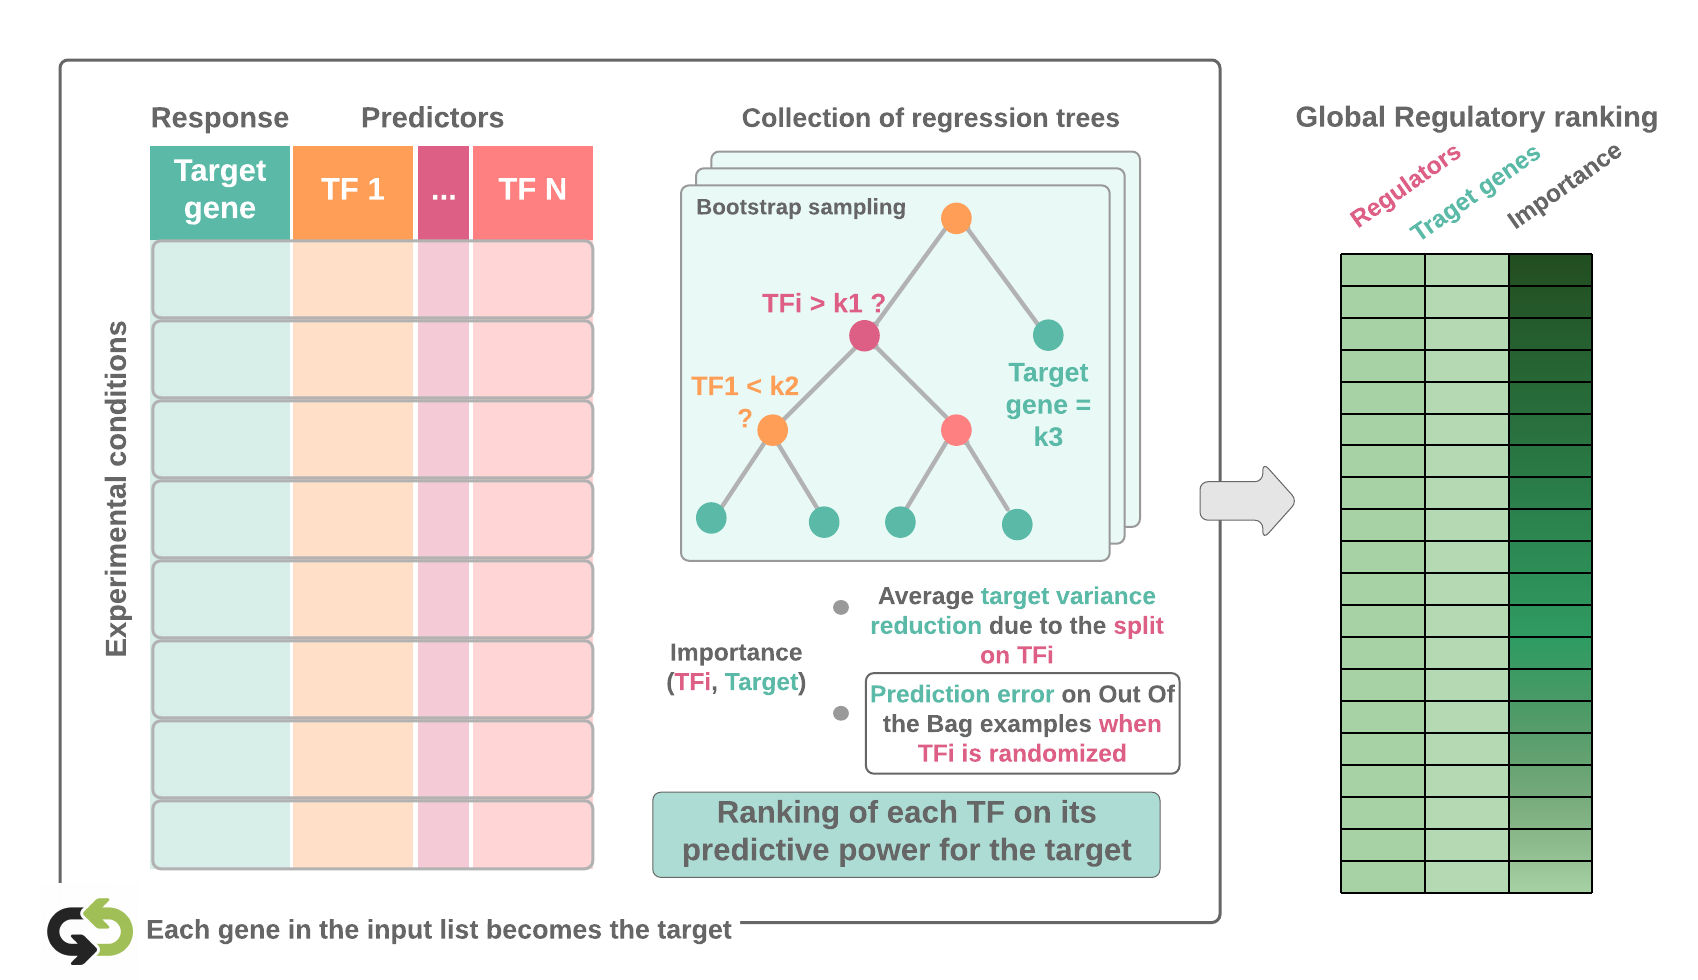
\includegraphics[scale = 0.38]{Figures/Regression/rf4.png}
    \end{overprint}
    \end{center}
\end{frame}




